
\documentclass{eecslides}

% \usecolortheme{RimouskiDark}

\usepackage[english]{babel}
\usepackage{lipsum}
\usepackage{graphicx}
\usepackage{caption}
\usepackage{hyperref}
\usepackage{xcolor}
\usepackage[round,authoryear]{natbib}
\usepackage[protrusion=true,expansion=true]{microtype}
\usepackage{booktabs}

\title[]{Data conservation - Perspectives, issues and solutions.}
\author[]{\color{white}  Miranda Bryant and Steve Vissault}
\website{\color{white} s.vissault@yahoo.fr}
\institute[\color{white} UQAR]{\color{white} \textbf{Les midis numériques}}
\date{ \color{white} \today}

\setbeamersize{text margin left=1cm} 
\setbeamersize{text margin right=1cm} 
\setbeamersize{text margin top=0.1cm} 

\begin{document}

\begin{frame}[plain]
\titlepage
\end{frame}


%%%%%%%%%%%%%%%%
\section{Introduction}
%%%%%%%%%%%%%%%%

\begin{frame}{Introduction}{Context}

All biologists collect data during their career but most of them are using \alert{inapropriate files}, called \textit{"flat files"}, to long term storage:

\begin{itemize}
	\item  Open Office or Microsoft spreadsheet
	\item  text and CSV files
\end{itemize}

\textbf{Some risks attributes at those practices:} Overwriting file, lost the full dataset or some records.

\end{frame}

%%%%%%%%%%%%%%%%%%%%%%%%%%%%%%%%%%%%%%%%%%%%%%%%%%%%%%%%

\begin{frame}{Introduction}{Context}

\textbf{\alert{Some disadvantage of classic storage file (i. e. Excel)}}

\begin{enumerate}
	\item No dynamic query, only filters
	\item Large dataset could be messy
	\item Exportability : Files corrupted, plateform could be different between users
	\item Absence of fonctionnality on manage multiple users
\end{enumerate}

%% Basic question for the public: How many people generate a dynamic cross table on Excel and got twice the same word because the first one start by a capital letter and the second doesn't start by a capital letter ?

%% Define briefly what's a medata file ?

\end{frame}

%%%%%%%%%%%%%%%%%%%%%%%%%%%%%%%%%%%%%%%%%%%%%%%%%%%%%%%%

\begin{frame}{Introduction}{Why do something different ?}


\begin{columns}[c]
	\begin{column}{.50\paperwidth}
		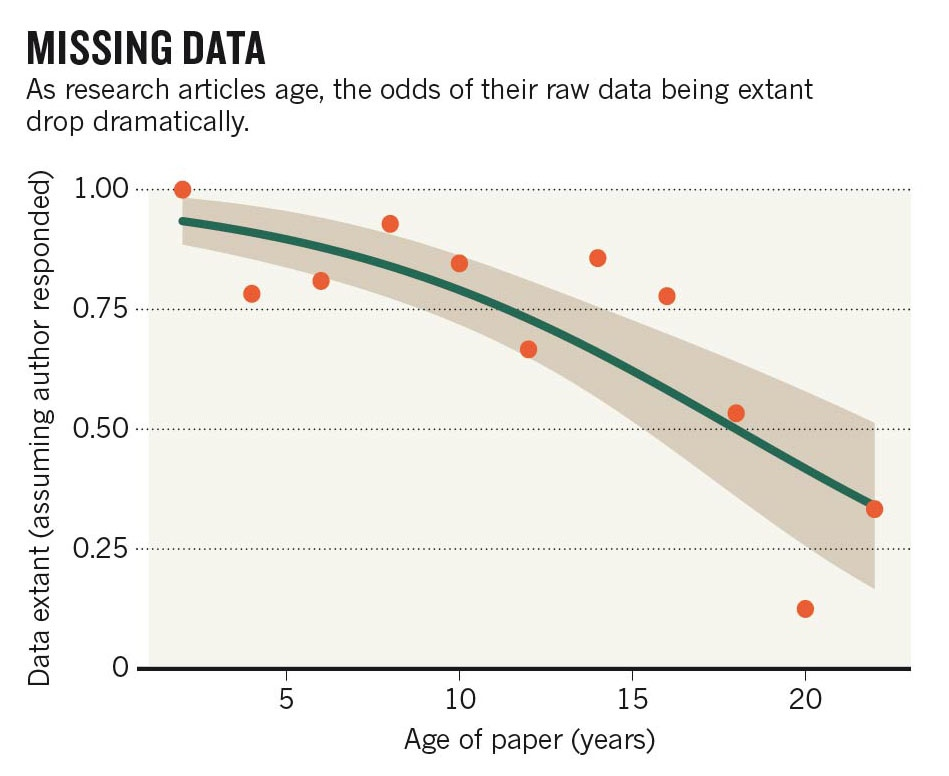
\includegraphics[width=.50\paperwidth]{Nature_fig.jpg}
	\end{column}
	\begin{column}{.4\paperwidth}
		 Data for almost all studies published just two years ago were still accessible, the chance of them being so \alert{fell by 17\% per year} \citep{Vines2013}
	\end{column}
\end{columns}

\end{frame}

%%%%%%%%%%%%%%%%%%%%%%%%%%%%%%%%%%%%%%%%%%%%%%%%%%%%%%%%


\begin{frame}{Introduction}{Why do something different ?}


\begin{columns}[c]
	\begin{column}{.50\paperwidth}
		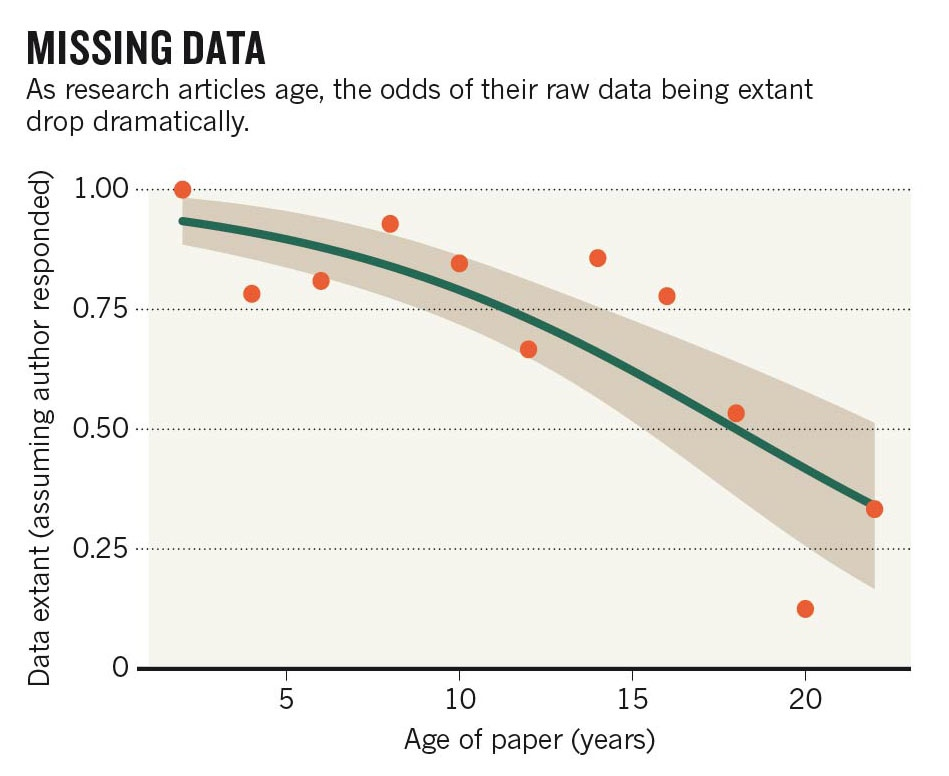
\includegraphics[width=.50\paperwidth]{Nature_fig.jpg}
	\end{column}
	\begin{column}{.4\paperwidth}
		\textbf{Why ?} Because researcher don't think about long term usability of storage data.
	\end{column}
\end{columns}

\end{frame}

%%%%%%%%%%%%%%%%%%%%%%%%%%%%%%%%%%%%%%%%%%%%%%%%%%%%%%%%

\begin{frame}{Introduction}{Why do something different ?}

\textbf{We need to keep focus on those points as a part of our biologist culture:}
	
	\begin{itemize}
		\item \alert{All datasets} containing specific information given a time and a location \alert{are usefull}.
		\item 80\% of datasets are built on \alert{public funding} \citep{Graham2013} and could be accessible publicly
		\item All datasets could be re-used, recycle or valorize (as the 3-R in waste management: Reduce, Reuse, Recycle) 
	\end{itemize}

	%% In this context, RDB could be a relevant solution for data in science

\end{frame}


%%%%%%%%%%%%%%%%%%%%%%%%%%%%%%%%%%%%%%%%%%%%%%%%%%%%%%%%

\begin{frame}{Introduction}{Why is a relational database a relevant solution for this context ?}
	
	\textbf{Most of Relational databases include:}
	\begin{itemize}
		\item \alert{\textbf{Metadata}}: Authors, Year of creation, columns type and description
			\begin{itemize}
				\item You ensure the happiness of users after 10 years of database no-used
			\end{itemize}
		\item \alert{\textbf{Connectivity}}: Users can get a remote secure access to your own data
			\begin{itemize}
				\item You keep the control localy on your data and manage users
			\end{itemize}
		\item \alert{\textbf{Exportability:}} User can request data from different platforms and languages (i. e. C, C++, R etc...)
		\item \alert{\textbf{Province:}} Store modifications and user-related data changes that allow for “roll back” or “updates” to the data
	\end{itemize}

	%% Following the previous context, RDB seems to be a great and adapted solution to solve our problems.

\end{frame}

%%%%%%%%%%%%%%%%%%%%%%%%%%%%%%%%%%%%%%%%%%%%%%%%%%%%%%%%

%%%%%%%%%%%%%%%%
\section{RDB}
%%%%%%%%%%%%%%%%

%%%%%%%%%%%%%%%%%%%%%%%%%%%%%%%%%%%%%%%%%%%%%%%%%%%%%%%%

\begin{frame}{Relational database}

\textbf{What is a Relational Database ?}
		 \begin{itemize}
			 \item A database is basically a Tables 
			\item A Table goes down a row of items and across many columns of attributes. The data can be organized into different tables.
			\item The tables have “relations” within and to each other
		 \end{itemize}

		\vfill

		\begin{center}
		 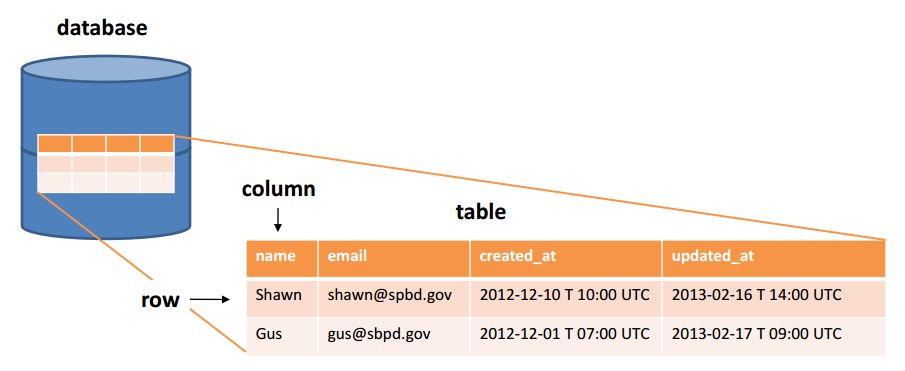
\includegraphics[width=.8\paperwidth]{relational-databases-for-dummies-fig1.png}
		\end{center}


	 %% Original text from Miranda: A Table goes down a row of items and across many columns of attributes (specific data descriptions). The data (along with new and different attributes) can be organized into different tables.

	%% Following the previous context, RDB seems to be a great and adapted solution to solve our problems.
\end{frame}

%%%%%%%%%%%%%%%%%%%%%%%%%%%%%%%%%%%%%%%%%%%%%%%%%%%%%%%%

\begin{frame}{Relational database}{What is a Relational Database ?}

\textbf{Four essential components:}
		 \begin{enumerate}
			 \item Row or Tuple : “A data set representing a single item” 
			\item Column: “A labeled element of a row” such an address, name, etc.
			\item Table: Contains data items in rows and columns
			\item Relationships : Links between tables (\textbf{See with Miranda})
		 \end{enumerate}

	\textbf{Each components is embedded in a design diagram}

%% This slide is perhaps a little bit redondant with all informations provide by the previous slide. See with Miranda.

\end{frame}

%%%%%%%%%%%%%%%%%%%%%%%%%%%%%%%%%%%%%%%%%%%%%%%%%%%%%%%%
%%% Slide missing: Table employees table. See with Miranda if that could be extract from the case study (Tree table instead of using employees table)
%%%%%%%%%%%%%%%%%%%%%%%%%%%%%%%%%%%%%%%%%%%%%%%%%%%%%%%%


%%%%%%%%%%%%%%%%%%%%%%%%%%%%%%%%%%%%%%%%%%%%%%%%%%%%%%%%
%%%%%%%%%%%%%%%%
\section{Design components}
%%%%%%%%%%%%%%%%
%%%%%%%%%%%%%%%%%%%%%%%%%%%%%%%%%%%%%%%%%%%%%%%%%%%%%%%%

\begin{frame}{Design components}{Usage of keys in table}

\alert{\textbf{Table contain keys:}}
		 \begin{description}
			 \item [Primary Keys] A key that is unique to the table to help identify a record
			\item [Composite Keys] A key that combines two or more columns to create a unique key into the table
		\end{description}

\end{frame}

%%%%%%%%%%%%%%%%%%%%%%%%%%%%%%%%%%%%%%%%%%%%%%%%%%%%%%%%

\begin{frame}{Design components}{Normalization}

\textbf{Some tricks to keep in mind about database normalization:}

		\begin{itemize}
			\item Do not have the “one file” or “one table” mentality
			\item If you have redundancy in your table, you need to think about normalization (multiple table design)
			\item Stages of normalization 1-5 NF (Normal Forms) are the most commonly accepted
			\begin{itemize}
				\item These are “technical”, but they describe the stages a database development will go through
			\end{itemize}
		\end{itemize}

\end{frame}

%%%%%%%%%%%%%%%%%%%%%%%%%%%%%%%%%%%%%%%%%%%%%%%%%%%%%%%%

\begin{frame}{Design components}{Relationships}

\textbf{Different type of relationship:}

		\begin{description}
			\item [1:1] Each key is linked with only one key in any other table
			\item [1:N] Each key in one table may be linked to many other keys in another table
			\item [N:N] One or more keys in a table can be linked to 0, 1, or many rows in another table
		\end{description}

\end{frame}


%%%%%%%%%%%%%%%%%%%%%%%%%%%%%%%%%%%%%%%%%%%%%%%%%%%%%%%%
%%%%%%%%%%%%%%%%
\section{Case studies}
%%%%%%%%%%%%%%%%
%%%%%%%%%%%%%%%%%%%%%%%%%%%%%%%%%%%%%%%%%%%%%%%%%%%%%%%%

\begin{frame}{Design components}{Relationships}

\centering
\textbf{Messy flat file example}

\end{frame}

%%%%%%%%%%%%%%%%%%%%%%%%%%%%%%%%%%%%%%%%%%%%%%%%%%%%%%%%

\begin{frame}{Design components}{Relationships}

\textbf{\alert{Need to be transform to a cleanest design without redundancy}}
\vspace{0.2cm}
	\begin{center}
		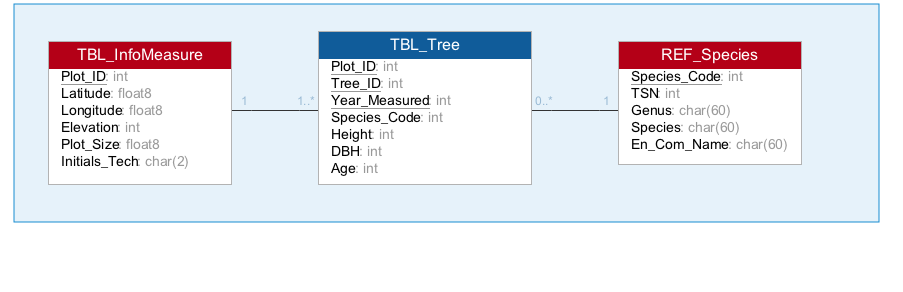
\includegraphics[width=0.8\paperwidth]{Ex1_pres_30Sept.png}
	\end{center}
\end{frame}

%%%%%%%%%%%%%%%%%%%%%%%%%%%%%%%%%%%%%%%%%%%%%%%%%%%%%%%%
%%%%%%%%%%%%%%%%
\section{RDB creation}
%%%%%%%%%%%%%%%%
%%%%%%%%%%%%%%%%%%%%%%%%%%%%%%%%%%%%%%%%%%%%%%%%%%%%%%%%

%%%%%%%%%%%%%%%%%%%%%%%%%%%%%%%%%%%%%%%%%%%%%%%%%%%%%%%%
%%%%%%%%%%%%%%%%
\section{QUICC-FOR}
%%%%%%%%%%%%%%%%
%%%%%%%%%%%%%%%%%%%%%%%%%%%%%%%%%%%%%%%%%%%%%%%%%%%%%%%%

%%%%%%%%%%%%%%%%%%%%%%%%%%%%%%%%%%%%%%%%%%%%%%%%%%%%%%%%
%%%%%%%%%%%%%%%%
\section{Conclusion}
%%%%%%%%%%%%%%%%
%%%%%%%%%%%%%%%%%%%%%%%%%%%%%%%%%%%%%%%%%%%%%%%%%%%%%%%%

%%%%%%%%%%%%%%%%
%% References
%%%%%%%%%%%%%%%%

\nocite{Poisot2013a}

\begin{frame}[allowsframebreaks]{References}
	\bibliographystyle{abbrvnat}
	\bibliography{/home/steve/Dropbox/Bibtex/OpenAccess}	
\end{frame}

\end{document}